\documentclass{article}
\usepackage[T1]{fontenc}
\usepackage{lmodern}
\usepackage{graphicx}
\usepackage{amsmath,amssymb}
\usepackage[a4paper,margin=2cm]{geometry}
\usepackage[absolute,overlay]{textpos}
\setlength{\TPHorizModule}{1mm}
\setlength{\TPVertModule}{1mm}
\usepackage[indonesian]{babel}
\usepackage{hyperref}
\setlength{\emergencystretch}{2em}
% unit: Halaman 47

\begin{document}

% === Halaman 47 (python/native) ===

47

Kriptanalisis Vigenere Cipher

• Friedrich Kasiski adalah orang yang pertama kali memecahkan 

Vigènere cipher pada Tahun 1863.

• Metodenya dinamakan metode Kasiski

Friedrich Kasiski 

Born: November 29, 1805 @ Schlochau, Kingdom of Prussia 

Died: May 22, 1881 (aged 75) @ Neustettin, German Empire 

Nationality: German

% deskripsi: gambar native xref 207
\noindent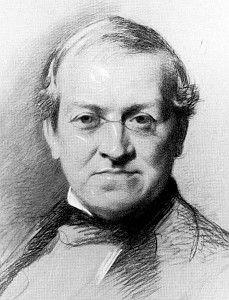
\includegraphics[width=0.85\textwidth]{../../images/python/page_047_img_01.jpeg}

\end{document}
